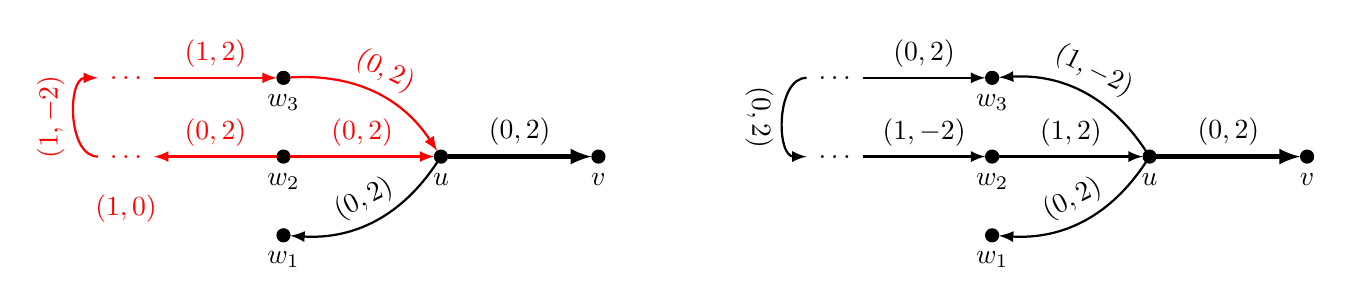
\begin{tikzpicture}[auto]

	\node (u) [circle, scale=0.5, fill, draw, label=below:$u$] at (0, 0) {};
	\node (v) [circle, scale=0.5, fill, draw, label=below:$v$] at (2, 0) {};
	\node (w1) [circle, scale=0.5, fill, draw, label=below:$w_1$] at (-2, -1) {};
	\node (w2) [circle, scale=0.5, fill, draw, label=below:$w_2$] at (-2, 0) {};
	\node (w3) [circle, scale=0.5, fill, draw, label=below:$w_3$] at (-2, 1) {};
	\node (dots1) [circle, red] at (-4, 1) {$\dots$};
	\node (dots2) [circle, red, label=below:\textcolor{red}{$\vv{(1,0)}$}] at (-4, 0) {$\dots$};

	\path[thick, -latex]
	(u) edge[ultra thick] node[sloped] {$(0,2)$} (v)
	(u) edge[bend left] node[sloped] {$(0,2)$} (w1)
	(w3) edge[bend left, red] node[sloped] {$(0,2)$} (u)
	(w2) edge[red] node[sloped] {$(0,2)$} (u)
	(dots1) edge[red] node[sloped] {$(1,2)$} (w3)
	(w2) edge[red] node[sloped] {$(0,2)$} (dots2)
	(dots2) edge[red, bend left=90] node[sloped] {$(1,-2)$} (dots1);
		
	\node (u') [circle, scale=0.5, fill, draw, label=below:$u$] at (9, 0) {};
	\node (v') [circle, scale=0.5, fill, draw, label=below:$v$] at (11, 0) {};
	\node (w1') [circle, scale=0.5, fill, draw, label=below:$w_1$] at (7, -1) {};
	\node (w2') [circle, scale=0.5, fill, draw, label=below:$w_2$] at (7, 0) {};
	\node (w3') [circle, scale=0.5, fill, draw, label=below:$w_3$] at (7, 1) {};
	\node (dots1') [circle] at (5, 1) {$\dots$};
	\node (dots2') [circle] at (5, 0) {$\dots$};

	\path[thick, -latex]
	(u') edge[ultra thick] node[sloped] {$(0,2)$} (v')
	(u') edge[bend left] node[sloped] {$(0,2)$} (w1')
	(u') edge[bend right] node[sloped] {$(1,-2)$} (w3')
	(w2') edge node[sloped] {$(1,2)$} (u')
	(dots1') edge node[sloped] {$(0,2)$} (w3')
	(dots2') edge node[sloped] {$(1,-2)$} (w2')
	(dots1') edge[bend right=90] node[sloped, below] {$(0,2)$} (dots2');

\end{tikzpicture}
